\chapter{Cosmic rays and the Pierre Auger Observatory}
\label{sec:uhecr}


\cite{Mollerach:2017idb}

%%%%%%%%%%%%%%%%%%%%%%%%%%%%%%%%%%%%
\section{Overview of cosmic rays}
\label{sec:uhecr:overview}

%%================================%%
\subsection{History}

-history: HESS, Auger and UHE

%%================================%%
\subsection{Energy spectrum}

%%%%%%%%%%%%%% SPEC SWORDY %%%%%%%%%%%%%%%
\begin{wrapfigure}{r}{0.55\textwidth}
  \centering
  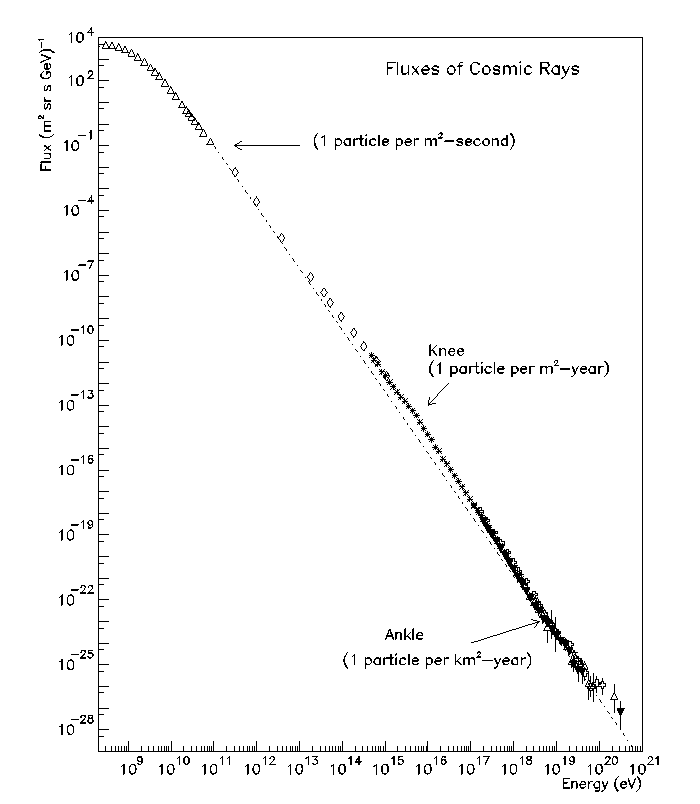
\includegraphics[width=0.55\textwidth]{spectrum_swordy}
  \caption{\cite{SwordyPlot2001}}
  \label{fig:uhecr:overview:spec:swordy}
\end{wrapfigure}

The cosmic rays flux as a function of its energy, the so called \emph{energy spectrum},
plays a central hole in the understanding of the astrophysical aspects behind these particles.
A compilation of measurements of the cosmic rays
energy spectrum over about 13 orders of magnitude
in energy is shown in~\cref{fig:uhecr:overview:spec:swordy}
One can see that from about \E{11} up to the highest energies
the spectrum can be described approximately 
by a power law $\text{d}\phi/\text{d}E \sim E^{-\gamma}$, where
the spectral index $\gamma$ is not exactly constant over all the energy range
but it changes only slightly between 2.5 and 3.2.
Because the cosmic rays spectrum extends over a very large
energy range, it is expected that different astrophysical mechanisms,
occuring at distinct scales, contribute to the origin
of the cosmic rays from different regions of the spectrum. As an illustration
we can point out that most of the modern models assume that the cosmic rays flux
is dominated by particles produced inside our galaxy up to around \e{17}-\E{18} and
an extragalactic origin for particles above this energy. The transition between
these two components is currently one of the most relevant topics of discussion.


Because of the spectrum steepness, the particle fluxes change over 27 orders of magnitude
from \e{11} and \E{21}. As indicated in~\cref{fig:uhecr:overview:spec:swordy},
while at \E{11} the flux is about 1 particle/m$^2$/second,
at \E{19} it drops to only 1 particle/km$^2$/year.
As a consequence, different experimental techniques have to be used to detect
cosmic ray particles at different energy ranges. Up to around \E{14}, the low flux
allows us to use small area instruments installed in ballons or satellites
to detects the particles before they interact with the earth's atmosphere.
Above this energy, the interaction with the atmosphere turns to be
useful since we can measure the cosmic rays indirectly through the detection of
the extensive air showers (see~\cref{sec:showers}). For that, large arrays of detectors
are used and their areas can vary substantially depending on the energy range they are
intended to study. As an example, the KASCADE experiment~\cite{\KASCADEPaper}
that is designed to measure particles from around \e{14} to \E{16}
has an area of 4000 m$^2$, while Pierre Auger
Observatory~\cite{\AugerPaper} has an area of 3000 km$^2$ to measure particles above \E{18}.

%%================================%%
\subsubsection{Main features of the energy spectrum}

The features of the cosmic ray spectrum are identified by the changes on the
spectral index $\gamma$. To better visualize these changes, we show
in~\cref{fig:uhecr:overview:spec:pdg} a compilation of measurements of
the spectrum from \E{13} in which the flux is scaled by a factor $E^{2.6}$.
As indicated in~\cref{fig:uhecr:overview:spec:pdg}, the first feature
is the so called \emph{first-knee} and it occurs around $3\times\E{15}$. At this energy
the index changes from $\gamma\approx 2.7$ to $3.0$. The next feature is
the \emph{second-knee}, around \E{17}, where there is a further steepening
and the index goes to $\gamma\approx 3.3$. The spectrum then becomes harder again
at the \emph{ankle}, around $5\times\E{18}$, where the index changes to $\gamma\approx 2.6$.
The final feature occurs at the highest energies, above $4\E{19}$, where the
value of the spectral index becomes very high ($>4$), caracterizing the so called
\emph{suppression}.


%%%%%%%%%%%%%% SPEC PDG %%%%%%%%%%%%%%%
\begin{figure}
  \centering
  
  \begin{overpic}[clip, rviewport=0 0 1 1,width=0.8\textwidth]{spectrum_pdg}
    \put(18,60){}
  \end{overpic}
  
  \caption{\cite{\PDGPaper}.}
  \label{fig:uhecr:overview:spec:pdg}
\end{figure}

The consistent interpretation of all these spectrum features requires the knowledge
about the composition of the cosmic rays. Particularly in the energy region compreending
the first and second-knee, very efficient composition measurements were performed
by KASCADE~\cite{\KASCADEPaper} and
KASCADE-Grande~\cite{\KASCADEGrandePaper} experiments. By using an experimental setup
that included surface detectors able to measured both number of charged particles and
number of muons in air showers, it was possible to measure the all particle spectrum
as well as to infer the spectra of individual groups of particles. In~\cref{}
we show the results of both experiments. Althought the final spectra are
strongly dependend on the hadronic interaction models
(see~\cref{sec:shower:simulations:models}) used in the analysis,
it is still possible to conclude that: (a) the first-knee is the result
of the suppression of the proton component of the spectrum~\cite{Antoni:2005wq},
(b) the suppression of the heavier components is consistent with
a rigidity dependent suppression~\cite{Antoni:2005wq} and (c) the second-knee coincides
with the suppression of the heaviest group of particles,
including iron nuclei~\cite{Apel:2011mi,Apel:2013uni}. 

Although the rigidity dependent suppression as an explanation for the knee
was a known hypothesis since it was suggested by Peters, in 1961~\cite{Peters1961},
the actual explanation is still a matter of discussion. The most simple
model would assume that the suppression is a consequence of a limit
in the maximum energy reachable by the sources~\cite{Gaisser:2013bla}.  
Alternative models include explanations based on the effect of the
drifting of cosmic rays in the galactic magnetic field~\cite{Ptuskin1993,Candia:2002qd}
and on the escape of cosmic rays from the galaxy~\cite{Giacinti:2014xya}.
Most of the models, however, converge on the fact that up to the second-knee
the cosmic ray flux is dominated by a galactic component. The transition
between this galactic and an extra-galactic component would then occur
at energies around the second-knee and the ankle.
The measurements and the models concerning this energy range (above \E{17}),
the range of interest of this thesis,
will be presented in~\cref{sec:uhecr:spectrum}.


%%================================%%
\subsection{Acceleration and sources}

The power-law shape of the energy spectrum indicates that
cosmic rays are not accelerated in thermal processes.
A stochastic acceleration mechanism was first proposed
by Fermi, in 1949~\cite{Fermi:1949ee}. The main idea is that
the multiple collisions of charged particles with moving magnetized regions
could accelerate them up to high energies. 
Althought a power law spectrum can be derived from this mechanism,
the overall acceleration efficiency is too low to explain the observed
energy density of cosmic rays. The average energy gain is given by $\Delta E/E\sim \beta^2$,
where $\beta = v/c$ and $v$ is the velocity of magnetic cloud.
Because of this second power of $\beta$, this mechanism is
called \emph{second order Fermi mechanism}.

A similar but more efficient mechanism was developed almost
two decades later~\cite{Axford1977,Krymsky1977,Bell:1978zc,Blandford:1978ky}.
The main idea now is that charged particles collide with multiple shock waves
and they gain energy by interacting with irregularities in the magnetic field.
The average energy gain is $\Delta E/E\sim \beta$ and again the power law energy
spectrum can be derived. The obtained spectral index is $\gamma=2-2.3$, which means that
propagation effects have to be responsible to account for the further speepning
of the observed spectrum.
This mechanism is called \emph{first order Fermi mechanism} or, alternatively,
\emph{diffusive shock acceleration}, and it is the basis of most of the models
that propose possible sources of cosmic rays.
A detailed approach on the diffusive shock acceleration theory can be found
in Ref.~\cite{Drury:1983zz} and a review on alternative acceleration
models in Ref.\cite{}.

The list of astrophysical objects usually considered as possible
acceleraton sites for cosmic rays includes neutron stars~\cite{Fang:2012rx},
active galactic nuclei~\cite{}, gamma ray burst~\cite{Vietri1995,Waxman:2004ez}
and others. A review of the candidates
for sources of cosmic rays can be found in Ref.~\cite{Torres:2004hk}.
Indenpendently of the details about the acceleration mechanisms in different
types of astrophysical enviroments, it is possible to estimate the maximum energy
that a certain type of object is able to accelerate particles. This was first done
by Hillas~\cite{Hillas1984} and the idea is simply consider that
the Larmos radius of the particles must be smaller than the size of the site
in which the particles are confined to be accelerated. As a reults one obtain that
\begin{equation}
  \frac{E_\text{max}}{\E{18}} \approx \frac{\beta Z}{2} \frac{B}{\mu\text{G}}\frac{L}{\text{kpc}},
\end{equation}
where $\beta$ is the tipical velocity of the shock waves in units of $c$, $Z$ is the charge
of the particles, $B$ is the magnectic field and $L$ is the tipical size of the site.
The graphical illustration of this relation is usually called \emph{Hillas-plot}.
We show one version of it, focused on the candidate sources of ultra-high energy
cosmic rays, in~\cref{fig:uhecr:overview:hillas}.
The diagonal lines show the cases of \E{20} proton and iron nuclei.

%%%%%%%%%%%%%% HILLAS PLOT %%%%%%%%%%%%%%%
\begin{figure}
  \centering
  
  \begin{overpic}[clip, rviewport=0 0 1 1,width=0.8\textwidth]{hillas}
    \put(18,60){}
  \end{overpic}
  
  \caption{\cite{Mollerach:2017idb}}
  \label{fig:uhecr:overview:hillas}
\end{figure}


Regarding cosmic rays of ultra-high energy, a famous family of models,
generically called \emph{top-down models}, assume that
they are not accelerated by astrophysical objects, but intead they are the products
of the decay of exotic super-massive particles. The origin of these exotic particles
could be, for example, topological defects from early Universe phase transition
of even dark matter. As a prediction of nearly all these models, a significant flux of
ultra-high energy photons should be observed. However, measurements
of Pierre Auger Observatory have shown that the actual flux is much lower than
the predictions~\cite{Aglietta:2007yx} and, therefore, the top-down hypothesis can be ruled out.
A review on the top-down models can be found in Ref.\cite{Olinto2000}.  


%%================================%%
\subsection{Propagation}
\label{sec:uhecr:overview:propagation}





%%%%%%%%%%%%%%%%%%%%%%%%%%%%%%%%%%%%
\section{Energy spectrum and composition at ultra-high energies}
\label{sec:uhecr:spectrum}

At the ultra-high energy range, two very evident features can be observed
in the spectrum: the ankle and the suppression. In~\cref{fig:uhecr:spectrum}
we show the most up to date spectrum as measured
by Pierre Auger Observatory~\cite{AugerSpec2017} and Telescope Array~\cite{TASpec2017},
where both features can be clearly seen. The ankle is a hardening of the spectrum
at $E\approx 5\times \E{18}$ which was first observed
in Haverah Park measurements in 1963~\cite{LinsleySpec1963}, and later confirmed
in measurements by AGASA~\cite{AgasaSpecPaper1995}, HiRes~\cite{\HiResSpecPaper},
Pierre Auger Observatory~\cite{Abraham:2008ru}
and Telescope Array~\cite{}. The suppression is an abrupt softning of the flux
at energies above $4\times \E{19}$ which was measured first by Hires~\cite{\HiResSpecPaper}
and later confirmed by Pierre Auger Observatory~\cite{Abraham:2008ru} and Telescope Array~\cite{}.
The fact that the suppression was not observed on the AGASA spectrum~\cite{Takeda:1998ps}
was a source of intense discussions along years. However,
it is currently accepted that the AGASA measurements are not trustful because
of systematical errors in the primary energy estimation~\cite{}.

%%%%%%%%%%%%%% SPEC UHECR %%%%%%%%%%%%%%%
\begin{figure}
  \centering
  
  \begin{overpic}[clip, rviewport=0 0 1 1,width=0.8\textwidth]{uhecr_spectrum}
    \put(18,60){}
  \end{overpic}
  
  \caption{\cite{AugerSpec2017,TASpec2017}.}
  \label{fig:uhecr:spectrum}
\end{figure}


The most precise inferences of the composition of cosmic rays
at this energy range are based on the \xmax measurements
performed by fluorescence telescopes in the modern experiments.
In~\cref{sec:shower:observables}, we present a detailed discussion about
the \xmax measurements, its composition interpretation, as well as
further measurements of air shower observables that could, in principle,
be used to infer composition. For now, it is only important to
point out that the cosmic rays composition
can be infered by comparing the measured \xmax distributions to
predictions obtained from air shower simulations. This procedure can be done
either by comparing only the moments of the \xmax distributions, which
gives only the average composition, or by comparing the whole distributions,
which can provide the abundances of individual groups of primaries.
In all cases, the composition interpretation is dependent on the
hadronic interaction model used to generate the simulation predictions.

Althought the energy spectrum with its both features can be sucesfully described
by multiple hypothesis, the composition measurements must be used to further constrain  
the models. Concerning the ankle, most of the models associate it to
the transition between the galactic and extra-galactic flux, which
can take place in energies between the second-knee and the ankle.
The composition predictions by these models can vary substantially depending
on the exact position of the transition and on the composition content of
the extra-galactic component. One historically relevant hypothesis to
describe the ankle without the galactic-to-extragalactic transition assumption is the
so called \emph{dip model}~\cite{Berezinsky:2002nc,Berezinsky:2005cq},
which proposes that the energy losses due to
pair production along the particle propagation would cause the hardening
of the spectrum around the ankle energies. It turns out that the success
of the dip model actually requires a nearly pure proton composition
around and above the ankle. Althought at the time of the model proposal
this composition assumption seemed to be fulfilled by the \xmax measurements
of HiRes experiments~\cite{\HiResXmaxPaper},
recent measurements of Pierre Auger Observatory
have proven it wrong~\cite{\AugerXmaxPRLPaper}.

Concerning the suppression, the two currently consided hypothesis
to explain it are the GZK effect (see~\cref{sec:uhecr:overview:propagation})
and the limit of the acceleration power by the sources. While the GZK hypothesis
require a composition dominated by protons at the highest energies, the source limit
would imply in a rigidity dependent suppression and consequently a increasingly heavier
composition as the energy increase. Similarly to what happened to the dip model,
the composition measurements by HiRes supported the GZK hypothesis for many year,
which was also changed after the Pierre Auger Observatory published its \xmax measurements
results. 

Many scenarios which propose to explain the ultra-high energy spectrum and composition
can be found in the
literature~\cite{Allard:2005cx,Aloisio:2011fv,Biermann:2011wf,Unger:2015laa,Globus:2015xga}.
Two features are commom to nearly all the recent models that are contrained by the
Auger \xmax measurements: the exact energy of the galactic-extragactic transition
(the energy in which both flux become equivalent) is around $1-4 \times \E{18}$
and the suppression is caused by a riditity dependent cutoff due to the limit
of the acceleration power of the sources. 
The absence of the GZK effect and its negative consequences
(e.g. the absence of correlation with nearby sources due to the deflection of
heavy nuclei in magnetic fields) have motivated the author of Ref.~\cite{Aloisio:2011fv}
to call this generic scenario of \emph{disappointing model}.

In a recent analysis done by Pierre Auger Collaboration,
the measured spectrum and the \xmax distributions were
jointly fitted by using simulations which account for
all the propagation effects~\cite{Aab:2016zth}.
We show in~\cref{fig:uhecr:combined} the results
of the fit by using the hadronic interaction model \EposLHCLong~\cite{\EposLHCPaper}
to simulate the \xmax distributions. The hypothesis of the limit of the acceleration power
by the sources as the source of the suppression is confirmed by the results of this analysis.
However, the lack of information about the composition given by the \xmax measurements
at energies above $4\times\E{19}$ is a limiting factor for this analysis, since the
spectrum is measured up to above \E{20}. Therefore, precise composition measurements
at the highest energies is a requirement to refine the interpretation
of the end of the cosmic rays spectrum. 

%%%%%%%%%%%%%% COMBINED FIT %%%%%%%%%%%%%%%
\begin{figure}
  \centering
  
  \begin{overpic}[clip, rviewport=0 0 1 1,width=0.9\textwidth]{combined_fit}
    \put(18,60){}
  \end{overpic}
  
  \caption{\cite{Aab:2016zth}.}
  \label{fig:uhecr:combined}
\end{figure}




%%%%%%%%%%%%%%%%%%%%%%%%%%%%%%%%%%%%
\section{The Pierre Auger Observatory}
\label{sec:uhecr:auger}


%%================================%%
\subsection{AugerPrime}






